

\section{Summary}
In this thesis we identified two classes of knowledge relevant to language
understanding: \textit{background} and \textit{contextual}.

We defined background knowledge as the implicit shared human knowledge that is
often omitted in human generated text or speech. We presented two ways to
incorporate this kind of knowledge in NLU systems.  In Chapter~\ref{chapter:ontolstm},
we explored how knowledge stated in an explicit symbolic knowledge base can be
incorporated in an NLU system to produce better encoded representations.
Particularly, we linked words to an ontology (WordNet),
and built an ontology-aware encoder that exploited the WordNet
hierarchies to learn context-sensitive token representations of words. We showed
the proposed model helps textual entailment and prepositional phrase attachment
tasks. By giving the encoder access to the hypernym paths of relevant concepts
we showed that we can learn useful task-dependent generalizations using an
attention mechanism.
Then in Chapter~\ref{chapter:nem}, we noted that not all background knowledge
can be stated symbolically, and focused on the kind of background knowledge that
is implicit in relations between linguistic elements. Concretely, we showed how selectional
preferences in structures relevant to the task at hand can be leveraged to
encode background knowledge. We showed that this is indeed more effective than
encoding whole sentences using comparable neural network architectures. 

We defined contextual knowledge as the explicit additional information that
reading comprehension systems need to ground reasoning in the respective
contexts. We focused on a subclass of reasoning tasks where reasoning can be
broken down into a sequence of discrete operations over structured contexts. We
viewed such problems as semantic parsing into domain-specific languages.
Given this framework, we pursued four research goals related to incorporating
contextual knowledge into semantic parsers, the first two related to the model
architecture while building transition based semantic parsers using neural encoder-decoder
models, and the remaining two related to the learning algorithms used when only weak
supervision is available. First, in Chapter~\ref{chapter:wikitables}, we investigated how the
knowledge of syntactic and semantic properties of the domain specific language
can be exploited to restrict the search space of the decoder in an
encoder-decoder model built for semantic parsing. Second, also in
Chapter~\ref{chapter:wikitables}, we dealt with the issue of reasoning over previously unseen
entities by using an entity linking module to score entity productions.
Then, in Chapter~\ref{chapter:nlvr} we dealt with the issue of spuriousness
while training weakly supervised semantic parsers. We incorporated minimal
lexicons into the parsers to define a measure of coverage, thereby ensuring that
the semantic parsers are penalized for producing logical forms that are not
relevant to the input utterances. Finally, we introduced a novel training scheme
that alternates between exploring the search space for new logical forms, and
maximizing the likelihood of the retrieved ones. We showed that this scheme
effectively exploits the compositionality of the logical form language to bias
the model towards good paths.
Using these techniques, we built parsers for two hard tasks: \WTQ{} and NLVR,
and showed state-of-the-art results on both tasks.

\section{Future work in Knowledge-Aware Encoding}
Following are some potential directions for future work that can be built on top
of the research ideas in Chapters~\ref{chapter:ontolstm} and~\ref{chapter:nem}.

We explored the use of a kind of symbolic knowledge, coming from an ontology, in
an end-to-end NLU system in Chapter~\ref{chapter:ontolstm}. This idea can be
extended to other NLU tasks while using appropriate knowledge sources.
For example, factual knowledge from Freebase may be helpful while building open
domain question answering systems, or knowledge from a protein interaction
database could be useful in building models that understand biomedical texts.
An important issue one needs to solve before doing so is linking. Mapping spans
in text to entities in a knowledge base, or entity linking, is very much an
unsolved problem. Similarly relation extraction, or identifying whether a given
span of text provides evidence for the existence of a specific relation that
could potentially exist between a pair of entities, is a very challenging
research problem. We did not have to deal with these issues completely in
Chapter~\ref{chapter:ontolstm}, because our entities there were synsets in
WordNet, and mapping them to relevant spans of text was relatively
straightforward. However, if we have to build similar systems with other
knowledge sources, we will have to build joint models for entity linking,
relation extraction, and reasoning, which is an exciting research direction.


In terms of incorporating implicit background into NLU systems, the ideas
in Chapter~\ref{chapter:ontolstm} form the basis for modeling only a specific
kind of commonsense: the eventive kind. More recent work has identified other
kinds of commonsense information: Examples include~\cite{forbes2017}, who
extract commonsense information related to physical properties of real world
objects, and~\cite{Tandon2018ReasoningAA} who encode commonsense information
related to state changes and procedures. In fact, identifying the kinds of
commonsense knowledge that is not readily available, encoded in some form, 
but those that NLU systems need for effective reasoning is a valuable exercise
in itself, and could pave way for solving several hard NLU tasks.

\section{Future work in Knowledge-Aware Reasoning}
In Chapters~\ref{chapter:wikitables} and~\ref{chapter:nlvr} we focused on a
specific subclass of reasoning tasks: those that are grounded in structured
contexts, and the reasoning can be expressed as a sequence of discrete
operations. There is a lot of ongoing work in tasks where the grounding is in
unstructured contexts such as paragraphs and
documents~\citep[among others]{hill2015goldilocks,Seo2016BidirectionalAF,dhingra2016gated,Xiong2016DynamicMN,yu2018qanet}.
To the best of our knowledge, all of that work performs reasoning with
continuous operations.
That may very well be because all these reasoning systems are built for datasets
like~\cite[among others]{Richardson2013MCTestAC,Rajpurkar2016SQuAD10,Joshi2017TriviaQAAL}
which require selecting spans in passages given as context.

One potential direction going forward is to define tasks
that require discrete reasoning over unstructured contexts, and build models for
them. To provide further motivation for this line of research, we will present
the result of a pilot annotation towards building such a dataset, and show some
empirical analysis from an initial model trained on that task.

\subsection{A challenging reasoning task}
As we have pointed out in Chapter~\ref{chapter:reasoning_related_work},
reasoning driven by discrete operations opens up a class of tasks that can be
modeled (e.g.:\ those that involve counting or sorting entities, performing set
operations, etc.). Reasoning for tasks such as these has been done by semantic
parsers in the past. However, semantic parsing typically operates on structured
data, where the entities and relations are explicitly identified, ideally as a
knowledge graph. Here, we introduce a new dataset where the contexts
are unstructured, and reasoning involves discrete operations. We present the
results of a pilot annotation study here, and comment on how this new dataset
calls for novel modeling choices.

\paragraph{Annotation task} The task was posted on Amazon Mechanical Turk, and the turkers were
asked to provide questions for paragraphs taken from Wikipedia where the answers
fall under one of three categories:
\begin{enumerate}
	\item A number that is not necessarily in the paragraph
	\item A date that is not necessarily in the paragraph
	\item A span either in the paragraph or the question 
\end{enumerate}
The annotators were asked to use counting, addition or subtraction, \textit{max}
or \textit{min} operations for answers that are numbers or dates. The annotation
task was designed such that any questions written by the annotators that can be
answered by the BiDAF~\citep{Seo2016BidirectionalAF}, a well performing
span selection model would be rejected. This procedure resulted in a dataset
that contains $17185$ questions in the training set, and $6861$ questions in the
development set, over $3124$ and $1100$ paragraphs respectively. We use this
dataset for our initial experiments below.

\begin{figure}
	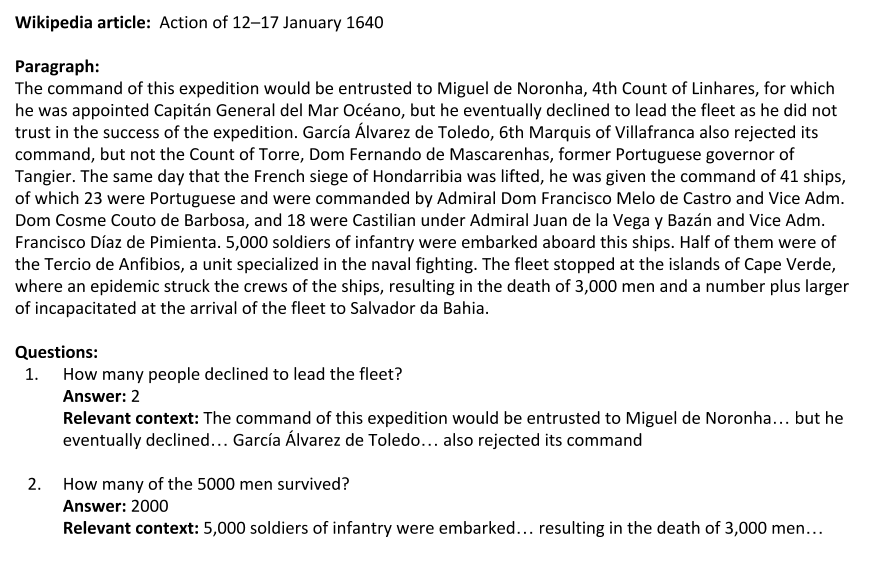
\includegraphics[width=\textwidth]{figures/drop_example.png}
	\caption{A hard reasoning task requiring discrete operations on
unstructured contexts}\label{fig:drop_example}
\end{figure}

Figure~\ref{fig:drop_example} shows an example paragraph along with two
associated questions that resulted from the pilot annotation task. As it can be
seen from the examples, it can seen that the questions at least require identifying entity types (e.g.
\textit{Miguel de Noronha} and \textit{Garcia Alvarez de Toledo} are of type
\textit{people}), solving co-reference over long distances (\textit{3000 men}
refers to a subset of \textit{5000 soldiers}), solving entailment (e.g.
\textit{death} contradicts \textit{survived}). Assuming all this information is
successfully extracted, the questions then require discrete operations (counting
for the first, and difference for the second).

\subsection{Towards building a semantic parser}
To assess the limitations of the techniques presented in this thesis, we applied
the parser we presented in Chapter~\ref{chapter:nlvr} to this task. A
prerequisite for doing so is to first extract relevant information from the
context to make a structure over which the parser can reason.

\paragraph{Information Extraction}
We run a trained open information extraction
(OpenIE) model~\citep{stanovsky2018supervised} over all the sentences in the
paragraph to extract predicate argument structures. This forms the base of our
knowledge graph, which is then augmented as follows: For each argument in each
predicate argument structure, we define additional relations from the text span
to all the numbers and entities (identified by a Named Entity Recognizer) in it.
Given this representation, we directly train a semantic parser using the
procedure described in Chapter~\ref{chapter:nlvr}: We run an exhaustive search
procedure to obtain logical forms for as many questions as possible, and train
an MML parser on it.

\paragraph{Results}
The exhaustive search procedure results in logical forms for only $50\%$ of the
training set, and on a manual inspection of a sample from them, we estimated
that only for $13\%$ of the questions, the search procedure could result in
logical form sets where at least one of the forms was correct. Finally, when the
MML model trained on this dataset had a $7.5\%$ accuracy on the development set.

\paragraph{Challenges}
The biggest hurdle in taking the route of semantic
parsing for this task is the lack of high-quality information extraction. Given that it is
already challenging to extract the kinds of information required by the
questions above, it would be even more difficult to build a semantic parser that
relies on the output of an IE system. One way to deal with this issue is to
train joint models for information extraction over paragraphs, and semantic
parsing over questions. This opens up a new class of NLP tasks where formalism
used for information extraction is determined by the end-task of question
answering.
